\documentclass[12pt]{article}    
\usepackage[arabic]{babel}       
\usepackage{amssymb}             
\usepackage{geometry}            
\usepackage{graphicx}            
\usepackage{wrapfig}             
\usepackage{amsmath}             
\usepackage{xcolor}              
\usepackage{polyglossia}         
\usepackage{tikz}                
\usetikzlibrary{arrows.meta, positioning, shapes, decorations.pathmorphing, decorations.text}                                       

% إعدادات الألوان
\definecolor{titleColor}{HTML}{800000} % Maroon for titles        
\definecolor{sectionColor}{HTML}{4682B4} % SteelBlue for sections 
\definecolor{textHighlight}{HTML}{DAA520} % Goldenrod for highlights                               
\definecolor{backgroundColor}{HTML}{FDF6E3} % Light beige background                               
\definecolor{frameColor}{HTML}{FFD700} % Golden frame                                              

% ضبط الخلفية
\pagecolor{backgroundColor}      
\color{black}                                                     

\begin{document}                                                                                   
% الزخارف العلوية والسفلية
\begin{tikzpicture}[remember picture, overlay]                        
    \node[anchor=north east, xshift=-0.5cm, yshift=-0.5cm] at (current page.north east) {};            
    \node[anchor=north west, xshift=0.5cm, yshift=-0.5cm] at (current page.north west) {};             
    \node[anchor=south west, xshift=0.5cm, yshift=0.5cm] at (current page.south west) {};              
    \node[anchor=south east, xshift=-0.5cm, yshift=0.5cm] at (current page.south east) {};         
\end{tikzpicture}                                                

\begin{center}                       
    \vspace*{0.5cm}                  
    {\Huge\textbf{\textcolor{titleColor}{السودان: الحرب والسلام، الاستقرار والازدهار}}}                 
    \vspace{0.5cm}                                                    
    {\large\textbf{\textcolor{sectionColor}{بابكر عثمان}}} \\         
    \vspace{0.2cm}                   
    {\today}                     
\end{center}                                                      

% إطار القصيدة
\begin{center}                   
    \begin{tikzpicture}              
        \node[rectangle, rounded corners, draw=frameColor, fill=white, thick, inner sep=0.5cm, text width=0.8\textwidth, align=center] {        
            \textbf{\Large إلى أختي وأخي، أطفال السبعينات، الآن أجداد} \\     
            \vspace{0.2cm}                   
            {\large                          
            يا طفولةَ السبعيناتِ في أمانِ \\
            نسجتُم الأملَ في قلبِ الزمانِ \\
            لعبتُم على الترابِ بلا قيودٍ \\
            وأحلامُكم كانت مثلَ الأماني \\                                      
            كانت الأيامُ تحنو بابتسامةٍ \\
            وساعاتُ النهارِ طُولُ الأماني \\
            لا هاتفَ يُلهي، لا شاشاتِ نورٍ \\
            بساطُ الأرضِ عالمكم بأمانِ \\                                        
            واليومَ قد كبرتم وزاد النورُ فيكم \\                                
            وأنتمُ الآنَ مصدرُ الألحانِ \\
            جدودٌ أنتم، وذِكرى الماضي حُلوةٌ \\                                  
            تُحكى للصغارِ بكل امتنانِ \\
            }                            
        };                               
    \end{tikzpicture}                
\end{center}                                                      

% صورة وتعليق
\begin{wrapfigure}{r}{0.40\textwidth}                             
    \rotatebox{0}{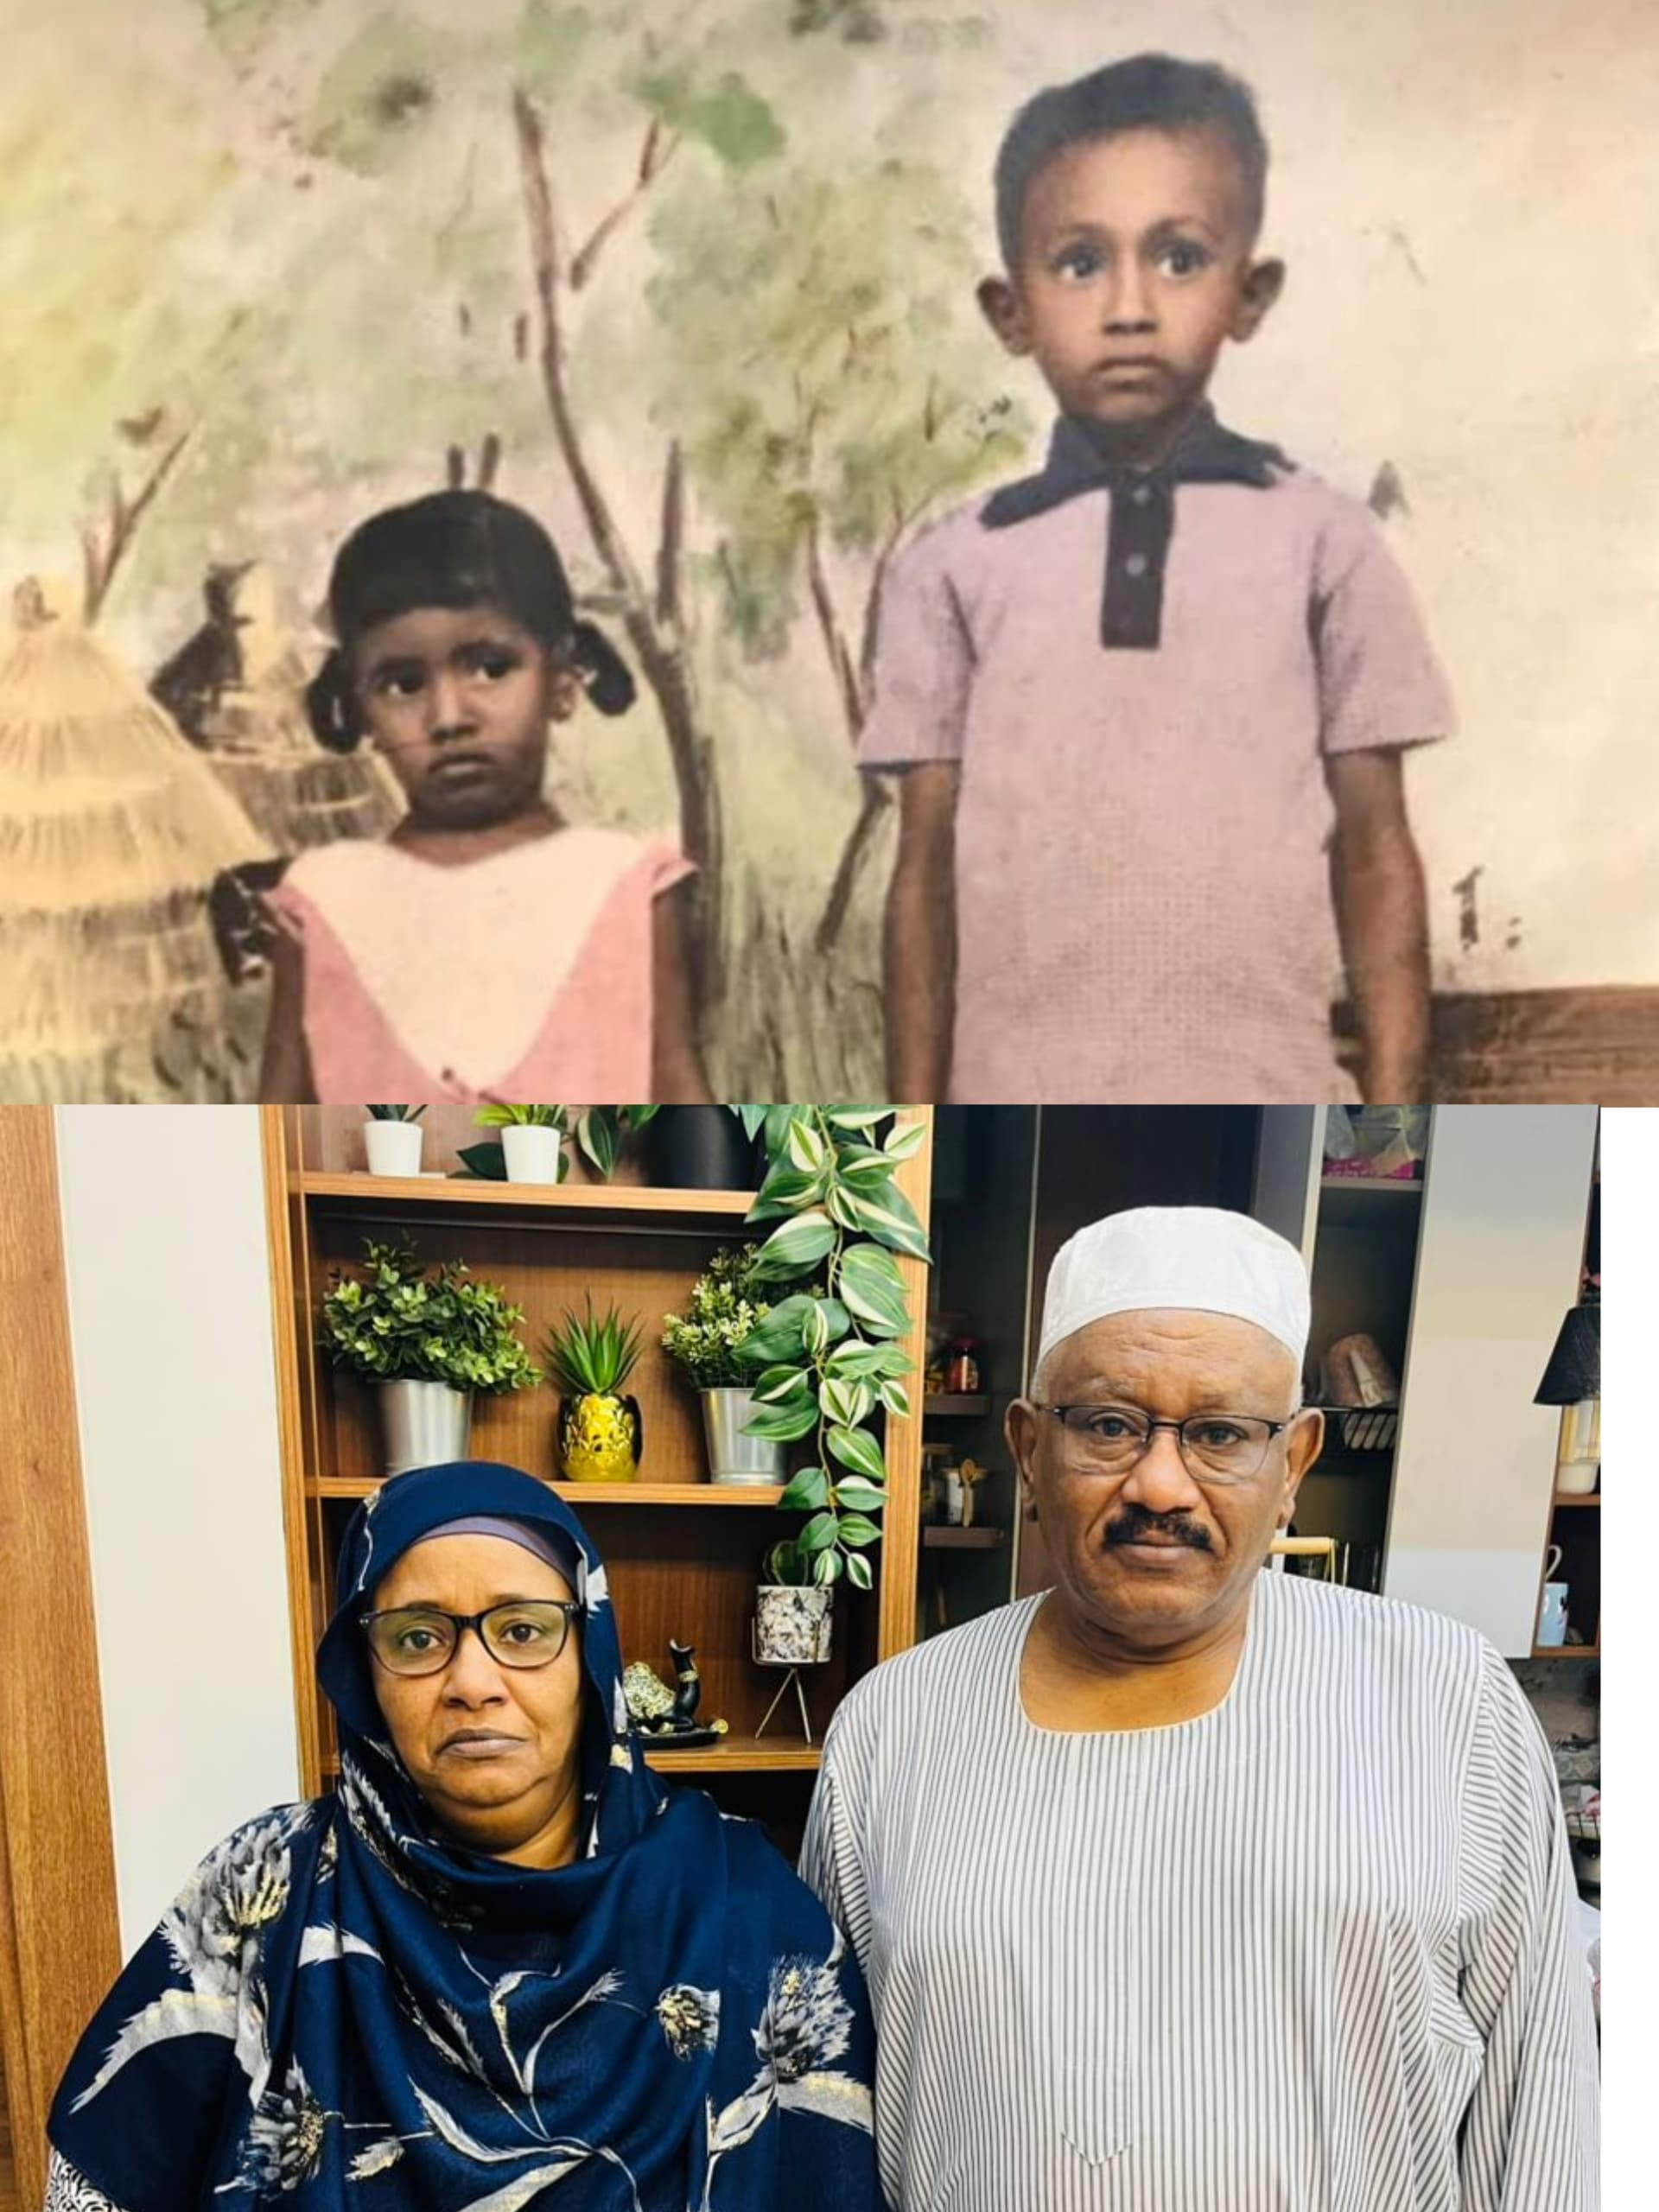
\includegraphics[width=0.4\textwidth]{205.jpg}}     
    \caption{\textcolor{sectionColor}{\small أطفال الماضي أجداد اليوم}}                                
\end{wrapfigure}                                                  

% المقطع الأخير
\noindent                        
{\textbf{\textcolor{textHighlight}{يا أختي، يا أخي، يا حكاياتِ الأمسِ}}} \\                          
حِكمتُكم تنيرُ الدربَ للزمانِ \\      
فالزمنُ يمضي، لكنَّ الأرواحَ باقيةٌ \\
تحملُ الحبَّ والوصلَ في المكانِ \\                                     
\textbf{أنتم تاريخُنا ومجدُنا الأصيلُ} \\                            
تعيشونَ في القلوبِ بكل ألوانِ \\    
فاحكوا حكاياكم للصغارِ دوماً \\    
علَّهم يروا العظمةَ في الإنسانِ.                                      

\end{document}

